% Chapter 1: Thesis Introduction
% This chapter provides an introduction to the thesis, including key definitions,
% research questions, and a summary of included papers.

\section{Introduction}
\subsection{Overview}

Industrial automation is undergoing a fundamental transformation driven by the shift from mass production to mass customization, requiring unprecedented levels of flexibility, reconfigurability, and adaptability in manufacturing systems. This evolution has been catalyzed by the emergence of modern computing technologies and their integration into industrial processes, leading to significant improvements in how industries operate. While early industrial automation focused primarily on cost reduction and productivity enhancement, contemporary systems must address complex challenges including quality assurance, system flexibility, reconfigurability, and component reusability. The control architecture of industrial automation systems has consequently evolved from centralized, monolithic designs to modular, decentralized component-based architectures that can adapt to changing production requirements.

The IEC 61499 standard has emerged as a cornerstone technology in this transformation, providing a vendor-independent, component-based framework for designing distributed control systems. This standard addresses the critical need for modular, reusable, flexible, extensible, scalable, and reconfigurable automation solutions. The IEC 61499 architecture is particularly well-suited for cyber-physical automation systems, where the integration of computational and physical processes creates complex interdependencies that traditional centralized control approaches cannot effectively manage. By enabling the development of distributed control applications through function blocks (FBs), IEC 61499 facilitates the creation of intelligent mechatronic components that can be seamlessly integrated and reused across different automation systems.

However, the increased complexity and distributed nature of these systems pose significant verification and validation (V\&V) challenges that traditional approaches cannot adequately address. While simulation remains a valuable tool for initial system testing and behavior assessment, it becomes increasingly inadequate as system complexity grows. Simulation alone cannot guarantee comprehensive validation of automation systems, particularly for safety-critical applications where the consequences of system failures can be severe. The limitations of simulation-based approaches include their inability to explore the entire state space of complex systems, their reliance on predefined test scenarios, and their inability to provide formal guarantees of system correctness.

To address these limitations, formal verification techniques have emerged as essential tools for ensuring system reliability and safety. Formal verification provides mathematically rigorous methods for proving or disproving the correctness of systems with respect to specified properties. Among these techniques, model checking has proven particularly valuable for industrial automation systems due to its automated nature, ability to generate counterexamples when properties are violated, and support for temporal logic specifications. Model checking systematically explores all reachable states of a system model to verify whether it satisfies given formal specifications, typically expressed in Computational Tree Logic (CTL) or Linear Temporal Logic (LTL).

Despite the theoretical advantages of formal verification, its practical adoption in industrial automation has been limited by several factors. The state-space explosion problem, where the number of possible system states grows exponentially with system complexity, presents a significant computational challenge. Additionally, the creation of formal models requires specialized expertise that is often not available in industrial engineering teams. The lack of user-friendly tools that integrate seamlessly into existing engineering workflows further hinders adoption. Furthermore, the gap between formal verification theory and practical industrial applications has created a barrier that prevents many automation engineers from leveraging these powerful techniques.

This thesis addresses these challenges by presenting a comprehensive framework that bridges the gap between formal verification theory and industrial practice. The research demonstrates how formal verification can be made accessible to automation engineers through integrated toolchains, automated model generation, and intuitive analysis tools. The framework leverages the IEC 61499 standard not only for controller design but also for modeling the system's physical environment (the "plant"), creating comprehensive closed-loop models suitable for rigorous verification.

A key innovation in this research is the introduction of non-deterministic transitions (NDTs) in plant models to enhance verification realism. Traditional deterministic plant models may fail to uncover timing-related bugs that occur only under specific timing conditions. By incorporating NDTs, the framework enables more realistic verification scenarios that can detect subtle, timing-dependent design flaws that would be difficult to identify through simulation alone. This approach allows verification engineers to selectively inject non-determinism where appropriate, enabling targeted formal verification under specific stress conditions.

The research also addresses the critical challenge of verifying runtime safety monitors, which are essential components in safety-critical systems. Runtime monitors observe system behavior during operation and signal errors when safety properties are violated. However, a monitor only improves system safety if its own correctness is guaranteed. The thesis presents a methodology for closed-loop model checking of monitors using non-deterministic twins of the controllers they supervise, ensuring that online safety mechanisms are themselves reliable.

Beyond formal verification, this research explores the application of process mining techniques to industrial control systems, representing a significant advancement in system understanding and model generation. Process mining, traditionally applied in business process management, has been adapted to address the unique challenges of industrial automation. The research demonstrates how process mining can extract control logic from event logs, enabling automated model generation for verification and analysis. This approach provides data-driven methods for understanding complex system behaviors and generating formal models from recorded event traces.

The research presents three complementary process mining approaches: process model extraction and conformance checking for anomaly detection, interactive learning for automatic controller generation, and automatic plant model generation for formal verification. These methodologies collectively address critical challenges in modern industrial automation, including the need for automated system understanding, the complexity of controller development, and the requirement for formal verification in safety-critical applications.

Another significant contribution of this research is the development of comprehensive cross-platform testing methodologies for IEC 61499 applications. Despite the standard's goal of enabling portability across different vendor platforms, practical implementation has revealed significant challenges due to variations in execution semantics and vendor-specific interpretations. The research addresses these challenges through systematic approaches to testing function blocks across different development and runtime environments, including comprehensive test function blocks for data types, boundary conditions, standard functions, and adapter support.

The research also explores model-based testing methodologies using service sequence models for test specification and automated generation. This approach provides a systematic method for ensuring consistent behavior across diverse vendor platforms, addressing a fundamental challenge in IEC 61499 adoption. The development of portable test applications that can execute across different IEC 61499 runtime environments represents a practical solution for comprehensive cross-platform validation.

The most transformative aspect of this research lies in the integration of emerging technologies—blockchain, large language models, and knowledge-driven AI agents—into industrial automation systems. The blockchain-enabled product traceability framework demonstrates how distributed ledger technology can enhance transparency and compliance in flexible manufacturing environments. By providing immutable, tamper-proof records of production processes, blockchain technology addresses the critical need for product traceability in modern manufacturing.

The integration of large language models (LLMs) into industrial control systems represents a significant advancement in human-machine interaction. LLMs enable operators to interact with complex systems using natural language, significantly reducing technical barriers and enhancing system accessibility. The research demonstrates how multi-actor LLM frameworks can provide sophisticated analysis and visualization capabilities for IEC 61499 control systems, enabling conversational AI interfaces that can handle complex queries and provide contextual recommendations.

The most significant advancement in this research is the development of knowledge-driven AI agents for planning, reasoning, and testing. These agents represent a paradigm shift in industrial automation, moving from rule-based systems to intelligent, adaptive systems that can understand natural language instructions, generate optimized operational plans, and autonomously validate system behavior. The agents leverage semantic reasoning with knowledge graphs to make context-aware decisions that balance operational efficiency with sustainability goals.

The AI agent framework includes specialized agents for planning, validation, and testing, demonstrating how complex industrial tasks can be decomposed and executed through coordinated AI systems. The planning agent generates optimized skill sequences to fulfill user-defined objectives by querying knowledge graphs and reasoning over operational constraints. The validating agent verifies whether proposed plans adhere to operational rules and resource constraints, while the testing agent supports requirement-based system testing by transforming specified requirements into executable test actions.

The integration of OPC UA communication enables these agents to interact directly with industrial control systems, reading real-time variables and executing control actions. This capability allows for dynamic decision-making based on sensor feedback, enabling systems to operate adaptively and improve efficiency by reducing unnecessary operations. The agents can handle complex scenarios such as conditional execution based on sensor feedback, enabling systems to adapt their behavior based on real-time conditions.

The research presented in this thesis addresses critical challenges in modern industrial automation while providing practical solutions that can be implemented in real-world systems. The integrated framework for formal verification makes powerful mathematical techniques accessible to automation engineers, while the process mining approaches provide data-driven methods for system understanding and model generation. The cross-platform testing methodologies ensure consistent behavior across diverse vendor platforms, and the AI-driven automation approaches enable intelligent, adaptive systems that can operate autonomously while maintaining high levels of reliability and efficiency.

The convergence of these technologies creates a comprehensive framework for the next generation of industrial automation systems. By integrating formal verification, process mining, cross-platform testing, and AI-driven automation, this research provides both theoretical foundations and practical tools for addressing the complex challenges facing modern manufacturing. The framework enables the development of intelligent, adaptive, and reliable industrial automation systems that can meet the demands of mass customization while maintaining high levels of safety and performance.

The research demonstrates that the integration of formal methods, AI, and industrial automation represents a promising direction for creating more efficient, reliable, and sustainable manufacturing systems. As industrial systems become increasingly complex and interconnected, the need for intelligent automation solutions will continue to grow. The research presented here provides the foundation for addressing these challenges while opening new avenues for future investigation and development.

The future of industrial automation lies in the seamless integration of human intelligence, artificial intelligence, and physical systems, creating cyber-physical systems that are not only efficient and reliable but also intelligent and adaptive. This thesis contributes to this vision by providing the theoretical foundations, practical tools, and experimental validation needed to realize truly intelligent industrial automation systems that can adapt to changing requirements and operate autonomously while maintaining high levels of safety and performance.

\section{Key Definitions}

Since many terms are used interchangeably by researchers in the field of industrial automation and formal verification, this section provides clear definitions of key technical terms used throughout this thesis. These definitions ensure non-ambiguous understanding of the terminology employed in this research.

\textbf{Abstract State Machine (ASM):} A mathematical model for describing the behavior of discrete dynamic systems. ASMs provide a formal foundation for modeling the execution semantics of IEC 61499 function blocks and serve as an intermediate representation in the translation process from IEC 61499 to formal verification languages.

\textbf{Architecture:} The fundamental organization of a system embodied in its components, their relationships to each other and to the environment, and the principles governing its design and evolution. In the context of industrial automation, architecture refers to the structural design of control systems and their constituent components.

\textbf{Blockchain:} A distributed, decentralized digital ledger technology that records transactions across multiple computers in a way that ensures security, transparency, and immutability. In industrial automation, blockchain technology is used for product traceability, process verification, and secure recording of manufacturing events.

\textbf{Closed-Loop Modeling:} A verification approach that includes both the controller and a model of the physical plant (environment) in the formal verification process. This approach constrains the inputs to the controller to only those that are physically possible, leading to more meaningful verification results.

\textbf{Conformance Checking:} A process mining technique that compares observed event logs against reference process models to identify deviations and ensure that system behavior conforms to expected specifications.

\textbf{Cyber-Physical System (CPS):} A system that integrates computational and physical processes, where embedded computers and networks monitor and control physical processes, usually with feedback loops where physical processes affect computations and vice versa.

\textbf{Digital Twin:} A virtual representation of a physical system that mirrors its real-world counterpart in real-time, enabling simulation, analysis, and optimization of system behavior.

\textbf{Event-Driven Architecture:} A software architecture pattern that promotes the production, detection, consumption, and reaction to events. In IEC 61499, function blocks communicate through events, making this architecture fundamental to distributed control systems.

\textbf{Execution Control Chart (ECC):} A state machine that defines the execution logic of a basic function block in IEC 61499. The ECC determines the sequence of algorithm execution in response to input events.

\textbf{Finite State Machine (FSM):} A mathematical model of computation that can be in exactly one of a finite number of states at any given time. FSMs are used to model the behavior of control systems and are fundamental to formal verification.

\textbf{Flexibility:} The ability of a system to adapt to new or different environments, requirements, or operational conditions without significant redesign or reconfiguration.

\textbf{Formal Methods:} Mathematical techniques for the specification, development, and verification of software and hardware systems. These methods provide rigorous, mathematical foundations for ensuring system correctness and reliability.

\textbf{Formal Verification:} The process of using mathematical methods to prove or disprove the correctness of a system with respect to a set of formal specifications. This includes techniques such as model checking, theorem proving, and static analysis.

\textbf{Function Block (FB):} A reusable software component in IEC 61499 that encapsulates data and algorithms. Function blocks interact through well-defined interfaces consisting of event and data inputs and outputs.

\textbf{Industrial Cyber-Physical System (iCPS):} A cyber-physical system specifically designed for industrial applications, integrating computational and physical processes in manufacturing and automation environments.

\textbf{Interoperability:} The ability to use multiple control hardware and software components from various vendors in a single application, ensuring seamless communication and integration.

\textbf{Knowledge Graph:} A structured representation of knowledge that captures relationships between entities in the form of nodes and edges. In AI-driven automation, knowledge graphs encode system configuration, available skills, and operational constraints.

\textbf{Large Language Model (LLM):} An artificial intelligence model trained on vast amounts of text data to understand and generate human language. LLMs are used in industrial automation for natural language processing, human-machine interaction, and intelligent analysis.

\textbf{Model Checking:} An automated formal verification technique that systematically explores all reachable states of a system model to verify whether it satisfies properties expressed in temporal logic.

\textbf{Multi-Agent System:} A system composed of multiple interacting intelligent agents that can work together to achieve complex objectives. In industrial automation, multi-agent systems enable distributed, flexible, and adaptive control.

\textbf{Non-Deterministic Transition (NDT):} A transition in a state machine that can fire at an arbitrary time after it becomes enabled. NDTs are used in plant models to represent execution uncertainties and enable more realistic verification scenarios.

\textbf{OPC UA (OPC Unified Architecture):} A machine-to-machine communication protocol for industrial automation that enables secure, reliable, and platform-independent data exchange between devices and systems.

\textbf{Plant Model:} A formal representation of the physical system or environment that a controller interacts with. Plant models are essential for closed-loop verification and enable comprehensive system analysis.

\textbf{Portability:} The usability of software across various environments, platforms, or runtime systems. In IEC 61499, portability refers to the ability to deploy function blocks across different vendor platforms.

\textbf{Process Discovery:} A process mining technique that automatically generates process models from event logs, revealing the actual behavior and workflow patterns of systems.

\textbf{Process Mining:} A data-driven approach to process analysis that extracts knowledge from event logs to understand, monitor, and improve processes. In industrial automation, process mining is used for system modeling, verification, and enhancement.

\textbf{Reconfigurability:} The ability of a system to be easily modified or adapted to accommodate changes in requirements, functionality, or operational conditions.

\textbf{Safety-Critical System:} A system whose failure could result in loss of life, significant property damage, or environmental harm. These systems require rigorous verification and validation to ensure reliability and safety.

\textbf{Service Sequence Model:} A standardized way to specify the expected input/output behavior of IEC 61499 function blocks, defining expected event occurrences, input values, and expected output values for test scenarios.

\textbf{Smart Contract:} A self-executing contract with predefined rules and conditions encoded in blockchain technology. Smart contracts automate predefined processes and ensure consistency and reliability in industrial applications.

\textbf{Specification:} A formal or informal description of system requirements, behavior, or properties. Specifications can be requirements specifications (used in requirements phases) or system specifications (used in design/development and testing phases).

\textbf{State Space Explosion:} A problem in formal verification where the number of possible system states grows exponentially with system complexity, making exhaustive verification computationally infeasible.

\textbf{Temporal Logic:} A formal system for reasoning about propositions qualified in terms of time. Linear Temporal Logic (LTL) and Computational Tree Logic (CTL) are commonly used in formal verification to specify system properties.

\textbf{Test-Driven Development (TDD):} A software development methodology that emphasizes writing tests before implementing functionality, ensuring that implemented behavior matches specified requirements from the beginning.

\textbf{Verification and Validation (V\&V):} Following IEEE Standard Glossary definitions, verification corresponds to determining if artifacts produced in the current phase fulfill requirements established during the previous phase. Validation is the process of evaluating software at the end of development to ensure compliance with requirements. Verification answers "Am I building the product right?" while validation answers "Am I building the right product?"

\section{List of Abbreviations}

This section provides a comprehensive list of abbreviations used throughout the thesis to ensure clarity and consistency in terminology.

\begin{itemize}
\item \textbf{4DIAC:} Framework for Distributed Industrial Automation and Control
\item \textbf{ASM:} Abstract State Machine
\item \textbf{BFB:} Basic Function Block
\item \textbf{CFB:} Composite Function Block
\item \textbf{CFBM:} Composite Function Block Module
\item \textbf{CORBA:} Common Object Request Broker Architecture
\item \textbf{CPS:} Cyber-Physical System
\item \textbf{CTL:} Computational Tree Logic
\item \textbf{ECC:} Execution Control Chart
\item \textbf{FB:} Function Block
\item \textbf{FBDK:} Function Block Development Kit
\item \textbf{FSM:} Finite State Machine
\item \textbf{HMI:} Human Machine Interface
\item \textbf{ICS:} Industrial Control System
\item \textbf{IPFS:} InterPlanetary File System
\item \textbf{KG:} Knowledge Graph
\item \textbf{LLM:} Large Language Model
\item \textbf{LTL:} Linear Temporal Logic
\item \textbf{NCES:} Net Condition/Event Systems
\item \textbf{NDT:} Non-Deterministic Transition
\item \textbf{NLP:} Natural Language Processing
\item \textbf{NuSMV:} New Symbolic Model Verifier
\item \textbf{OPC UA:} OPC Unified Architecture
\item \textbf{PLC:} Programmable Logic Controller
\item \textbf{RAG:} Retrieval Augmented Generation
\item \textbf{RMCSES:} Reference Model of Control/Sensor Events Sequencing
\item \textbf{RTE:} Runtime Environment
\item \textbf{SDLC:} Software Development Life Cycle
\item \textbf{SIFB:} Service Interface Function Block
\item \textbf{SMC:} State Machine Component
\item \textbf{SMV:} Symbolic Model Verifier
\item \textbf{SQL:} Structured Query Language
\item \textbf{TDD:} Test-Driven Development
\item \textbf{UML:} Unified Modeling Language
\item \textbf{V\&V:} Verification and Validation
\item \textbf{XES:} eXtensible Event Stream
\end{itemize}

\section{Research Question}
\subsection{Aims \& Objectives}
The objective of this research is to enhance formal verification in industrial automation by incorporating modular nondeterministic transitions (NDTs) to improve realism and complexity management. It aims to develop modular applications with automatic verification procedures and automate plant model generation within IEC 61499 for formal verification. Additionally, the research focuses on creating portable test codes for cross-platform validation to ensure consistency in different runtime environments. To further optimize industrial automation, the study integrates AI agents to enable reasoning, planning, and real-time adaptability of IEC 61499-based control systems.

\subsection{Hypothesis}
This research hypothesizes that integrating formal verification techniques with modular automation frameworks enhances system reliability and scalability, while non-deterministic transitions enable realistic simulation and validation of complex processes. Process mining can extract control logic from event logs, enabling automated model generation for verification and analysis. Automated test generation improves system portability and validation, ensuring reliable cross-platform performance. AI-driven agents, leveraging knowledge graphs and LLMs, enhance industrial automation by enabling sustainable planning, dynamic execution, and requirement-based validation of IEC 61499 control systems through OPC UA integration.

\subsection{Problem Statement}
Integrating formal verification into the design of IEC 61499-based automation systems remains a challenge in ensuring reliability and correctness. Leveraging process mining to generate formal models from event logs can improve system analysis, but effective methods for this transformation are needed. Detecting portability issues before deployment is critical to prevent failures due to execution environment differences. AI-driven reasoning, planning and decision-making can enhance system adaptability, but efficient implementation methods need further exploration.

\subsection{Research Questions}
\subsubsection{Main Research Question}
How can best practices in formal verification, process mining, model-based testing, and AI-driven automation be combined to enhance the safety, conformance, portability and adaptability of industrial control systems?

\subsubsection{Sub-questions}
\begin{enumerate}
    \item How can formal verification techniques be applied to modular industrial automation systems to ensure their safety and correctness?
    
    \item How can the plant model creation be automated by process mining? How could such models be integrated into the formal verification toolchain to verify and optimize industrial control systems based on IEC 61499?
    
    \item How can model-based testing improve the portability and reliability of IEC 61499 control applications across multiple platforms?
    
    \item How can a knowledge-driven AI agent interpret natural-language operator instructions to generate sustainable execution plans for IEC 61499-based industrial control systems? How can AI agents automate requirement-based testing and validate system behavior to ensure conformance in industrial control systems?
\end{enumerate}

\section{Included Papers' Summary}
The following section lists all publications included in Part II of the thesis. A short summary of each paper is presented and my contribution is highlighted. Figure~\ref{fig:ch1:research_mapping} shows the mapping between papers appended and what research question they address and Figure~\ref{fig:ch1:paper_relationship} shows how the appended papers are linked to achieving the thesis objective.

\begin{figure}[H]
    \centering
    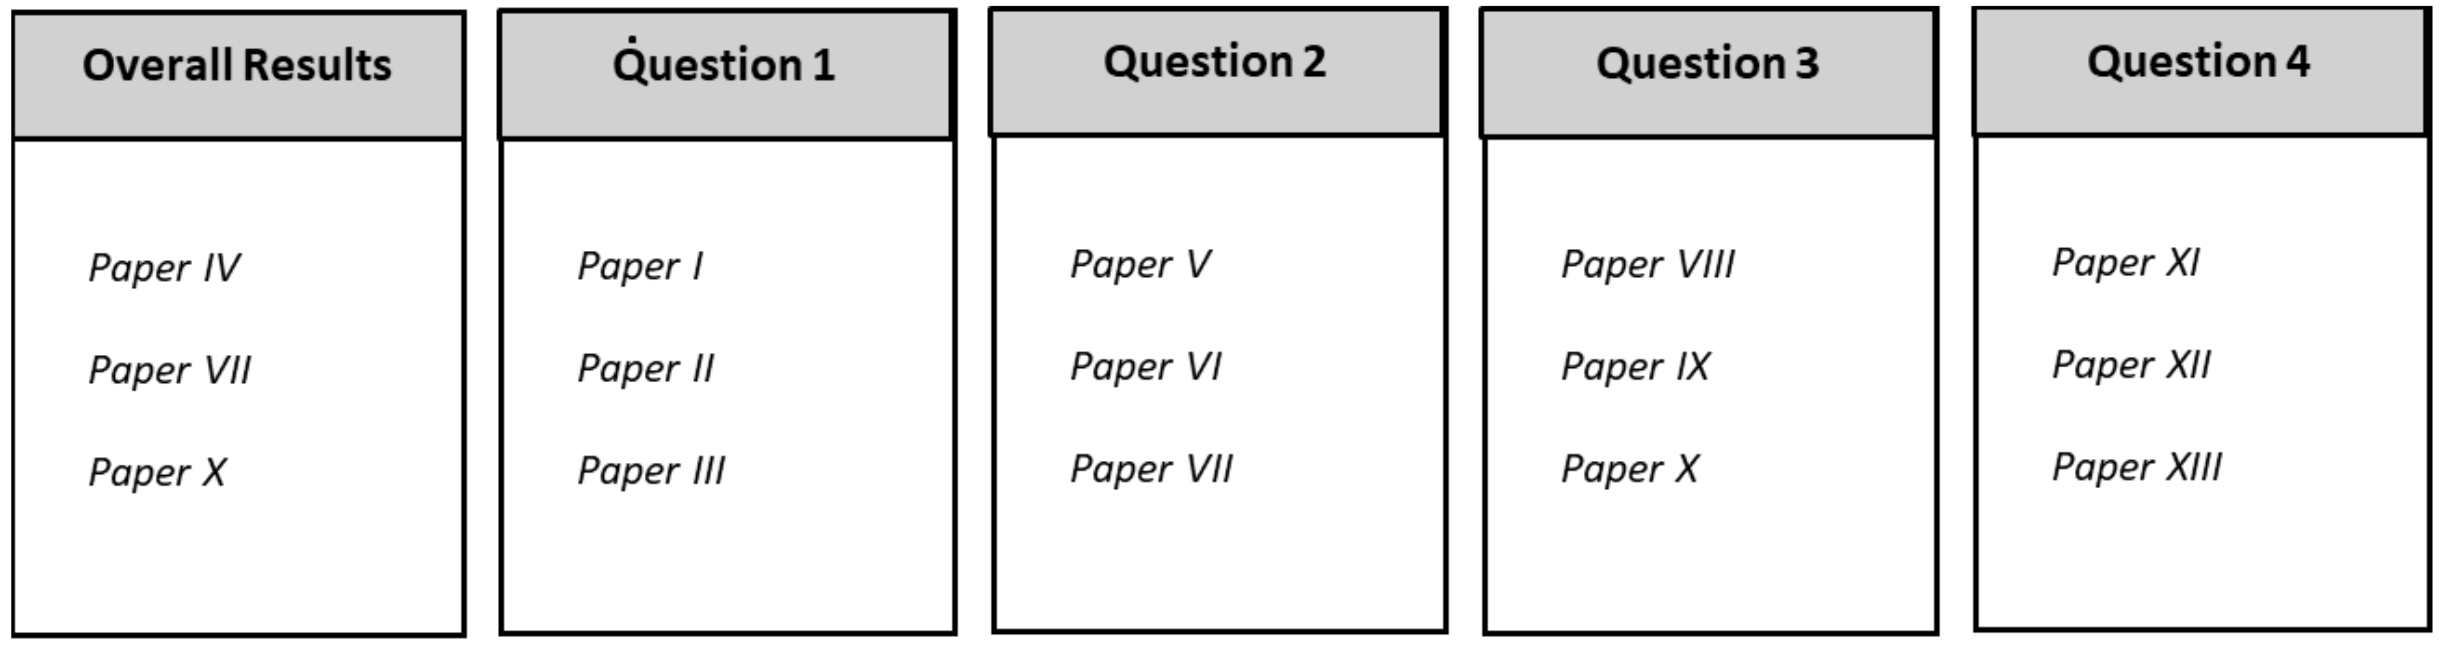
\includegraphics[width=0.75\textwidth]{chapters/images/chapter1/relationship_papers_researchquestions.png}
    \caption{Mapping between research questions and appended papers.}
    \label{fig:ch1:research_mapping}
\end{figure}

\begin{figure}[H]
    \centering
    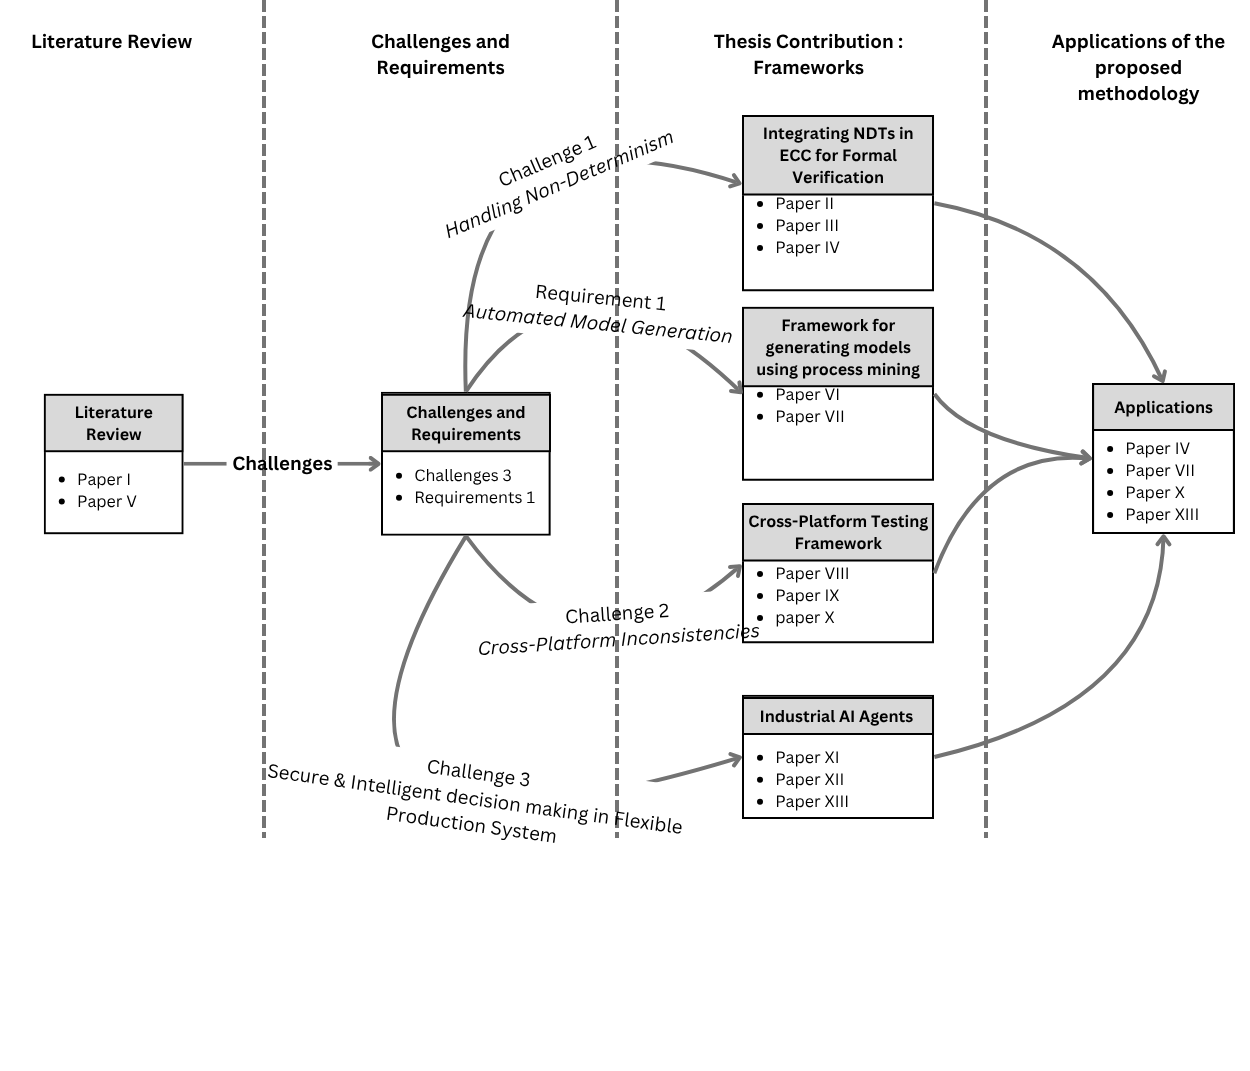
\includegraphics[width=0.75\textwidth]{chapters/images/chapter1/Literature Review.png}
    \caption{Relation between appended papers and the thesis topics.}
    \label{fig:ch1:paper_relationship}
\end{figure}

\subsection{Paper A}
\textbf{\textit{Title:}} Formal Modelling, Analysis, and Synthesis of Modular Industrial Systems Inspired by Net Condition/Event Systems\\
\textbf{\textit{Authors:}} Midhun Xavier, Sandeep Patil, Victor Dubinin, and Valeriy Vyatkin\\
\textbf{\textit{Published in:}} Lecture Notes in Computer Science (LNCS), 2023\\
\textbf{\textit{Summary:}} This paper summarises recent developments in the application of modular formalisms to model-based verification of industrial automation systems. The paper is a tribute to the legacy of Professor Hans-Michael Hanisch who invented Net Condition/Event Systems (NCES) and passionately promoted the closed-loop modelling approach to modelling and analysis of automation systems. The paper surveys the related works and highlights the impact NCES has made on the current progress of modular automation systems verification.\\

\subsection{Paper B}
\textbf{\textit{Title:}} Cyber-physical automation systems modelling with IEC 61499 for their formal verification\\
\textbf{\textit{Authors:}} Midhun Xavier, Sandeep Patil, and Valeriy Vyatkin\\
\textbf{\textit{Published in:}} 2021 IEEE 19th International Conference on Industrial Informatics (INDIN), Palma de Mallorca, Spain, 2021, pp. 1-6, doi: 10.1109/INDIN45523.2021.9557416\\
\textbf{\textit{Summary:}} Distributed industrial automation systems pose a significant challenge for their efficient verification and validation due to their heterogeneous structure, use of wireless communication and decentralised logic. The inherent inter twinning of computational and communication processes with complex physical dynamics has called for the term cyber-physical systems (CPS) to emphasize the challenges and the need for new development approaches. The {IEC 61499} architecture is getting increasingly recognised as a powerful mechanism for engineering such systems. It has been proven also as an efficient way of modeling CPS in automation. The challenge of IEC 61499 verification has been well-recognized from the early stages of the standard's development and evaluation. Closed-loop modelling has been proposed for the most comprehensive verification, which implies the need for modelling the plant. In quite many works, the plant modelling was done in the same formalism, which was used eventually to represent the model for the model-checker. Graphical modelling languages of finite-state machines and Petri nets were used in particular, and the models were prepared using the corresponding graphical editors. However, the IEC 61499 itself provides a graphical engineering interface and supports programming in terms of state machines. Therefore, a problem-oriented notation could be proposed to take advantage of the existing tools and avoid using additional ones in the process of modelling. This paper proposes such an approach by introducing a tool chain.\\

\subsection{Paper C}
\textbf{\textit{Title:}} Formal verification of observers supervising a cyber-physical system implemented using IEC 61499\\
\textbf{\textit{Authors:}} Polina Ovsiannikova, Etienne Le Priol, Vincent Perret, Pranay Jhunjhunwala, Midhun Xavier, and Valeriy Vyatkin\\
\textbf{\textit{Published in:}} 2023 IEEE 32nd International Symposium on Industrial Electronics (ISIE), Helsinki, Finland, 2023, pp. 1-6, doi: 10.1109/ISIE51358.2023.10228148\\
\textbf{\textit{Summary:}} A rigorous check is a significant phase in the design process of control programs of safety-critical cyber-physical systems. Here, we consider such programs to be implemented using IEC~61499 standard for industrial automation. After the check is performed (for example, using formal verification), the engineer needs to ensure that even in unexpected situations, the system will not fail during the runtime, and for this online verification methods can be utilized. In this work, we consider attaching monitors implemented as basic function blocks to the interface of the controller, thus having a property being monitored represented in the form of a state machine. Now, monitors make the system safer only if their quality is also ensured. Since their complexity is far lower than the complexity of the controller, they can be model checked, however, in the case of IEC~61499 function blocks, open-loop model checking will produce spurious counterexamples as it will allow combinations that are not possible according to the IEC~61499 function blocks semantics (e.g., data transferred without firing the event). The current work addresses this issue and proposes a method for close-loop model checking of monitors, using the non-deterministic twin of a controller under supervision. We present our approach using the system of two orthogonal pneumatic cylinders.\\

\subsection{Paper D}
\textbf{\textit{Title:}} Formal Verification of the Control Software of a Radioactive Material Remote Handling System, Based on IEC 61499\\
\textbf{\textit{Authors:}} Giordano Lilli, Midhun Xavier, Etienne Le Priol, Vincent Perret, Tatiana Liakh, Roberto Oboe, and Valeriy Vyatkin\\
\textbf{\textit{Published in:}} IEEE Open Journal of the Industrial Electronics Society, vol. 4, pp. 417-431, 2023, doi: 10.1109/OJIES.2023.3321084\\
\textbf{\textit{Summary:}} Automation systems within nuclear laboratories are intended to work under harsh operating conditions. SPES (Selective Production of Exotic Species) is a nuclear research facility currently under construction by INFN (Istituto Nazionale di Fisica Nucleare), dedicated to the production and study of Radioactive Ion Beams (RIBs). Isotopes are produced within the Target Ion Source (TIS) unit, a vacuum vessel that must be replaced on a regular basis. The highly radioactive environment necessitates the deployment of a set of automated systems dedicated to the unit's remote management. To meet high-level security standards, the design of such instrumentation and control systems must include extensive verification. Based on specific safety requirements, model checking can be used to assess the systems' correctness. This paper describes how to employ an integrated tool-chain to design, simulate, formally verify, and deploy the control software for the Horizontal Handling Machine, a safety-critical remote handling system in operation at SPES. The IEC 61499 standard's adoption led to a redesign of the control logic. Following a preliminary online simulation, the closed-loop system has been formally verified using the NuSMV symbolic model checker, with the help of the FB2SMV converter. Additionally, the FBME tool was used for automating verification and analyzing counterexamples.\\

\subsection{Paper E}
\textbf{\textit{Title:}} Process mining in industrial control systems\\
\textbf{\textit{Authors:}} Midhun Xavier, Victor Dubinin, Sandeep Patil, and Valeriy Vyatkin\\
\textbf{\textit{Published in:}} 2022 IEEE 20th International Conference on Industrial Informatics (INDIN), Perth, Australia, 2022, pp. 1-6, doi: 10.1109/INDIN51773.2022.9976111\\
\textbf{\textit{Summary:}} In this paper, we discuss how process mining techniques can be applied in industrial control systems for modeling, verification, and enhancement of the cyber-physical system based on recorded data logs. Process mining is used for extracting the process models in different notations from the recorded behavioral traces of the system. The output model of the system's behavior is mainly derived using an open-source tool called ProM. The model can be used for such applications as anomaly detection, detection of cyber-attacks and alarm analysis in industrial control systems with the help of various control flow discovery algorithms. The extracted process model can be used to verify how the event log deviates from it by replaying the log on Petri net for conformance analysis.\\

\subsection{Paper F}
\textbf{\textit{Title:}} An interactive learning approach on digital twin for deriving the controller logic in IEC 61499 standard\\
\textbf{\textit{Authors:}} Midhun Xavier, Victor Dubinin, Sandeep Patil, and Valeriy Vyatkin\\
\textbf{\textit{Published in:}} 2022 IEEE 27th International Conference on Emerging Technologies and Factory Automation (ETFA), Stuttgart, Germany, 2022, pp. 1-7,\\ doi: 10.1109/ETFA52439.2022.9921602\\
\textbf{\textit{Summary:}} In this paper, we describe a method to automatically derive the controller for an automated process by an interactive learning approach using a simulation model developed in Visual Components 3D simulation software. The latter is used to record the events of the processes and the controller is generated as an IEC 61499 function block. To create different process scenarios, the actuator signals are triggered manually in appropriate order. The controller logic in Petri net is derived by process discovery algorithms with help of recorded events and conversion of Petri net to IEC 61499 function blocks is done by a software tool configured with a set of transformation rules.\\

\subsection{Paper G}
\textbf{\textit{Title:}} A Framework for the Generation of Monitor and Plant Model From Event Logs Using Process Mining for Formal Verification of Event-Driven Systems\\
\textbf{\textit{Authors:}} Midhun Xavier, Victor Dubinin, Sandeep Patil, and Valeriy Vyatkin\\
\textbf{\textit{Published in:}} IEEE Open Journal of the Industrial Electronics Society, vol. 5, pp. 517-534, 2024, doi: 10.1109/OJIES.2024.3406059\\
\textbf{\textit{Summary:}} This paper proposes a method for the automatic generation of a plant model and monitoring using process mining algorithms based on recorded event logs. The behavioural traces of the system are captured by recording event logs during plant operation in either manual control mode or with an automatic controller. Process discovery algorithms are then applied to extract the logic of the process behaviour properties from the recorded event logs. The result is represented as a Petri net, which is used to construct the state machine of the plant model and monitor and is in accordance with the IEC 61499 standard. The monitor is implemented as a function block and can be deployed in real time to trigger an error signal whenever there is a deviation from the actual process scenario. The plant model and controller are connected in a closed loop and are used for the formal verification of the system with the help of the 'fb2smv' converter and symbolic model checking tool NuSMV.\\

\subsection{Paper H}
\textbf{\textit{Title:}} Developing a Test Suite for Evaluating IEC 61499 Application Portability\\
\textbf{\textit{Authors:}} Midhun Xavier, Sandeep Patil, and Valeriy Vyatkin\\
\textbf{\textit{Published in:}} 2023 IEEE 32nd International Symposium on Industrial Electronics (ISIE), Helsinki, Finland, 2023, pp. 1-4, doi: 10.1109/ISIE51358.2023.10228154\\
\textbf{\textit{Summary:}} This paper presents the creation of a series of function blocks with the specific aim of testing the portability of IEC 61499 applications across diverse development and runtime environments. These function blocks have been developed to cover a wide range of test scenarios, including basic data types, functions, boundary conditions, and adapter features. The function blocks can be conveniently exported or imported through the use of XML files, thus facilitating seamless testing. By testing the runtime environment of different IEC 61499 systems, these function blocks help to identify and highlight any possible issues that may arise related to portability.\\

\subsection{Paper I}
\textbf{\textit{Title:}} Generating Portable Test Cases for IEC 61499 FBs from Interface Behaviour Specifications\\
\textbf{\textit{Authors:}} Midhun Xavier, Sandeep Patil, and Valeriy Vyatkin\\
\textbf{\textit{Published in:}} 2023 IEEE 28th International Conference on Emerging Technologies and Factory Automation (ETFA), Sinaia, Romania, 2023, pp. 1-4,\\ doi: 10.1109/ETFA54631.2023.10275633\\
\textbf{\textit{Summary:}} IEC 61499 is an executable, event-based language for control software that allows visual and textual implementation of individual software components (Function Blocks, FBs). The standardized visual service sequence model specifies the expected input/output behaviour of a component, thus supporting model-based testing. We present our approach for testing an FB on various platforms, which helps manage the variations in execution semantics between different vendors. First, service sequences are generated manually or derived from an existing (partial) implementation. Then, these service sequences serve as unit tests for this implementation. Finally, we create a test application that is executable on any IEC 61499-compliant platform. Executing tests directly in the target platform helps validate the correct functionality of an FB before deploying the control software to a cyber-physical system.\\

\subsection{Paper J}
\textbf{\textit{Title:}} Develop Once, Test Everywhere: Cross-Platform Development of Distributed Control Software\\
\textbf{\textit{Authors:}} Bianca Wiesmayr, Melanie Winter, Midhun Xavier, Sandeep Patil, Valeriy Vyatkin, and Alois Zoitl\\
\textbf{\textit{Published in:}} IEEE Open Journal of the Industrial Electronics Society, 2025 [Not Yet Published]\\
\textbf{\textit{Summary:}} Realising flexible industrial automation systems requires an approach for autonomous and distributed designs. Programmable Logic Controllers (PLCs) are the established platform for real-time control software that accesses sensors and actuators. Standards play an important role in distributed automation, for instance, IEC~61131-3 and IEC~61499, which define programming paradigms for control software development. Multiple interacting PLCs form a distributed control system. Providing the respective engineering methodologies and models is a goal of IEC~61499. Heterogeneous systems can even be composed of PLCs from various vendors and programmed with different tools. Furthermore, a single development tool can distribute control code across multiple runtime environments (RTEs), motivating the need to execute component tests in each of these RTEs. Developers of IEC~61499 library modules will also need to provide their modules to users of various development environments. Despite the focus on portability and the standardized XML format for data exchange, IEC~61499-based software components must often be modified during the porting process. Due to varying execution behaviour, the ported software may behave differently on each platform, possibly leading to malfunctions of the distributed control system. Therefore, it is crucial to thoroughly test an IEC 61499 application on each relevant target platform before using the software in a real-world system. A platform-independent test specification has the potential to greatly reduce the involved effort.\\

\subsection{Paper K}
\textbf{\textit{Title:}} Enhancing Traceability in Flexible Production System: A Blockchain-Powered Approach in IEC 61499 Multi-Agent Control System\\
\textbf{\textit{Authors:}} Midhun Xavier, Sandeep Patil, and Valeriy Vyatkin\\
\textbf{\textit{Published in:}} 2024 IEEE 33rd International Symposium on Industrial Electronics (ISIE), Ulsan, Korea, Republic of, 2024, pp. 1-6, doi: 10.1109/ISIE54533.2024.10595680\\
\textbf{\textit{Summary:}} This paper presents a novel approach for tracking products and processes within industrial multi-agent control systems by leveraging blockchain technology. The suggested solution facilitates the recording and validation of every step involved in creating a tailored product through the utilization of Ethereum-based smart contracts. The OWL ontology is used to describe agents and their capabilities and these software agents interact with IEC 61499 function blocks for process execution. The software agents record process events at each stage on the blockchain and the latter smart contract helps to trace and verify these process sequences of the customised product.\\

\subsection{Paper L}
\textbf{\textit{Title:}} LLM-Powered Multi-Actor System for Intelligent Analysis and Visualization of IEC 61499 Control Systems\\
\textbf{\textit{Authors:}} Midhun Xavier, Sandeep Patil, and Valeriy Vyatkin\\
\textbf{\textit{Published in:}} IECON 2024 - 50th Annual Conference of the IEEE Industrial Electronics Society, Chicago, IL, USA, 2024, pp. 1-8, doi: 10.1109/IECON55916.2024.10905502\\
\textbf{\textit{Summary:}} This paper introduces an innovative multiactor framework that harnesses the potential of LLMs to augment the functionalities of ICS. By integrating conversational AI technologies, this framework significantly improves human-machine interactions, enabling sophisticated analysis and visualization of intricate data sets. The core of the system comprises specialized LLM actors that interact through a LangGraph-based multi-actor framework, addressing various aspects of IEC 61499 control systems including PLC code analysis, SQL query execution, and data visualization. This integration enables operators to interact with the control system using natural language, significantly reducing technical barriers and enhancing the accessibility and usability of complex industrial systems.\\

\subsection{Paper M}
\textbf{\textit{Title:}} ReACT - Gen AI Agents for Reasoning, Planning, and Testing in Industrial Automation Systems\\
\textbf{\textit{Authors:}} Midhun Xavier, Sandeep Patil, and Valeriy Vyatkin\\
\textbf{\textit{Published in:}} [Not Submitted]\\
\textbf{\textit{Summary:}} This paper proposes a novel AI agent for reasoning, planning, and testing industrial automation applications. The AI agent accepts operator instructions in natural language and performs semantic reasoning over functional requirements to generate an optimized cost-effective action plan. This plan comprises a sequence of executable actions that can be deployed in industrial control systems (ICS) to enable efficient and sustainable machine operation. Then the AI agent automates the testing of control systems by comparing the agent's planned and executed actions against expected outputs, ensuring requirement conformance and enhancing system reliability. Experimental results demonstrate the effectiveness of the AI agent in generating sustainable operational plans and validating control system behavior for laboratory scale case studies, underscoring its potential in the future of intelligent industrial automation.\\
